\documentclass[conference]{IEEEtran}
\usepackage{amsmath}
\usepackage{booktabs}
\usepackage{graphicx}
\usepackage{microtype}
\usepackage{url}
\usepackage{tikz}
\usetikzlibrary{arrows.meta}
\usepackage{algorithm}
\usepackage{algorithmic}
\graphicspath{{figures/}}
% generated by experiments/make_paper_numbers.py - do not edit
\newcommand{\nAudLeakyFullA}{28.6}
\newcommand{\nAudLeakyFullB}{20.3}
\newcommand{\nAudLeakyFullC}{31.0}
\newcommand{\nAudLeakyGenA}{0.0}
\newcommand{\nAudLeakyGenB}{0.0}
\newcommand{\nAudLeakyGenC}{0.0}
\newcommand{\nAudLeakyLogitA}{36.7}
\newcommand{\nAudLeakyLogitB}{31.5}
\newcommand{\nAudLeakyLogitBestA}{36.7}
\newcommand{\nAudLeakyLogitBestB}{34.6}
\newcommand{\nAudLeakyLogitBestC}{29.4}
\newcommand{\nAudLeakyLogitC}{19.8}
\newcommand{\nAudLeakyPermPA}{0.011}
\newcommand{\nAudLeakyPermPB}{0.114}
\newcommand{\nAudLeakyPermPC}{0.011}
\newcommand{\nAudLeakyRidgeA}{33.9}
\newcommand{\nAudLeakyRidgeB}{21.1}
\newcommand{\nAudLeakyRidgeC}{31.5}
\newcommand{\nAudPrimaryFullA}{12.8}
\newcommand{\nAudPrimaryFullB}{11.5}
\newcommand{\nAudPrimaryFullC}{11.5}
\newcommand{\nAudPrimaryGenA}{0.0}
\newcommand{\nAudPrimaryGenB}{0.0}
\newcommand{\nAudPrimaryGenC}{0.0}
\newcommand{\nAudPrimaryLogitA}{11.2}
\newcommand{\nAudPrimaryLogitB}{10.7}
\newcommand{\nAudPrimaryLogitBestA}{13.3}
\newcommand{\nAudPrimaryLogitBestB}{14.3}
\newcommand{\nAudPrimaryLogitBestC}{14.6}
\newcommand{\nAudPrimaryLogitC}{11.2}
\newcommand{\nAudPrimaryPermPA}{0.422}
\newcommand{\nAudPrimaryPermPB}{0.809}
\newcommand{\nAudPrimaryPermPC}{0.618}
\newcommand{\nAudPrimaryRidgeA}{14.3}
\newcommand{\nAudPrimaryRidgeB}{10.2}
\newcommand{\nAudPrimaryRidgeC}{12.2}
\newcommand{\nAudUntreatedFullA}{50.8}
\newcommand{\nAudUntreatedFullB}{63.0}
\newcommand{\nAudUntreatedFullC}{61.7}
\newcommand{\nAudUntreatedGenA}{0.0}
\newcommand{\nAudUntreatedGenB}{0.0}
\newcommand{\nAudUntreatedGenC}{0.0}
\newcommand{\nAudUntreatedLogitA}{99.7}
\newcommand{\nAudUntreatedLogitB}{99.7}
\newcommand{\nAudUntreatedLogitBestA}{99.7}
\newcommand{\nAudUntreatedLogitBestB}{99.7}
\newcommand{\nAudUntreatedLogitBestC}{99.7}
\newcommand{\nAudUntreatedLogitC}{99.7}
\newcommand{\nAudUntreatedPermPA}{0.010}
\newcommand{\nAudUntreatedPermPB}{0.010}
\newcommand{\nAudUntreatedPermPC}{0.010}
\newcommand{\nAudUntreatedRidgeA}{70.3}
\newcommand{\nAudUntreatedRidgeB}{69.5}
\newcommand{\nAudUntreatedRidgeC}{63.3}
\newcommand{\nAuditExactA}{8}
\newcommand{\nAuditExactB}{8}
\newcommand{\nAuditExactC}{8}
\newcommand{\nAuditSeedsA}{8}
\newcommand{\nAuditSeedsB}{8}
\newcommand{\nAuditSeedsC}{8}
\newcommand{\nBatchExactA}{5}
\newcommand{\nBatchExactB}{5}
\newcommand{\nBatchExactC}{5}
\newcommand{\nBatchMarginHiA}{37}
\newcommand{\nBatchMarginHiB}{20}
\newcommand{\nBatchMarginHiC}{24}
\newcommand{\nBatchMarginLoA}{37}
\newcommand{\nBatchMarginLoB}{17}
\newcommand{\nBatchMarginLoC}{23}
\newcommand{\nBatchNA}{5}
\newcommand{\nBatchNB}{5}
\newcommand{\nBatchNC}{5}
\newcommand{\nBurstZeroA}{16.5}
\newcommand{\nBurstZeroB}{40.8}
\newcommand{\nBurstZeroC}{81.9}
\newcommand{\nCacheMBA}{1.41}
\newcommand{\nCacheMBB}{3.75}
\newcommand{\nCacheMBC}{7.50}
\newcommand{\nCfdRandomDistA}{0.049}
\newcommand{\nCfdRandomDistB}{0.054}
\newcommand{\nCfdRandomDistC}{0.070}
\newcommand{\nCfdRandomDistF}{0.048}
\newcommand{\nCfdRandomGenIdA}{41.7}
\newcommand{\nCfdRandomGenIdB}{52.4}
\newcommand{\nCfdRandomGenIdC}{44.7}
\newcommand{\nCfdRandomGenIdF}{42.9}
\newcommand{\nCfdRandomKlA}{0.0115}
\newcommand{\nCfdRandomKlB}{0.0129}
\newcommand{\nCfdRandomKlC}{0.0194}
\newcommand{\nCfdRandomKlF}{0.0114}
\newcommand{\nCfdResetDistA}{0.410}
\newcommand{\nCfdResetDistB}{0.477}
\newcommand{\nCfdResetDistC}{0.506}
\newcommand{\nCfdResetDistF}{0.410}
\newcommand{\nCfdResetGenIdA}{0.7}
\newcommand{\nCfdResetGenIdB}{0.1}
\newcommand{\nCfdResetGenIdC}{2.2}
\newcommand{\nCfdResetGenIdF}{0.7}
\newcommand{\nCfdResetKlA}{0.7899}
\newcommand{\nCfdResetKlB}{0.8041}
\newcommand{\nCfdResetKlC}{0.4402}
\newcommand{\nCfdResetKlF}{0.7899}
\newcommand{\nCfdSeedsA}{3}
\newcommand{\nCfdSeedsB}{3}
\newcommand{\nCfdSeedsC}{3}
\newcommand{\nCfdSeedsF}{3}
\newcommand{\nCfdShadowDistA}{0.000}
\newcommand{\nCfdShadowDistB}{0.000}
\newcommand{\nCfdShadowDistC}{0.000}
\newcommand{\nCfdShadowDistF}{0.000}
\newcommand{\nCfdShadowGenIdA}{100.0}
\newcommand{\nCfdShadowGenIdB}{100.0}
\newcommand{\nCfdShadowGenIdC}{100.0}
\newcommand{\nCfdShadowGenIdF}{100.0}
\newcommand{\nCfdShadowKlA}{-0.0000}
\newcommand{\nCfdShadowKlB}{-0.0000}
\newcommand{\nCfdShadowKlC}{-0.0000}
\newcommand{\nCfdShadowKlF}{-0.0000}
\newcommand{\nCfdSubspaceDistA}{0.048}
\newcommand{\nCfdSubspaceDistB}{0.054}
\newcommand{\nCfdSubspaceDistC}{0.070}
\newcommand{\nCfdSubspaceDistF}{0.060}
\newcommand{\nCfdSubspaceGenIdA}{43.2}
\newcommand{\nCfdSubspaceGenIdB}{52.5}
\newcommand{\nCfdSubspaceGenIdC}{44.6}
\newcommand{\nCfdSubspaceGenIdF}{35.4}
\newcommand{\nCfdSubspaceKlA}{0.0110}
\newcommand{\nCfdSubspaceKlB}{0.0131}
\newcommand{\nCfdSubspaceKlC}{0.0192}
\newcommand{\nCfdSubspaceKlF}{0.0144}
\newcommand{\nCfdUntreatedDistA}{0.047}
\newcommand{\nCfdUntreatedDistB}{0.054}
\newcommand{\nCfdUntreatedDistC}{0.070}
\newcommand{\nCfdUntreatedDistF}{0.047}
\newcommand{\nCfdUntreatedGenIdA}{42.8}
\newcommand{\nCfdUntreatedGenIdB}{52.1}
\newcommand{\nCfdUntreatedGenIdC}{43.8}
\newcommand{\nCfdUntreatedGenIdF}{42.8}
\newcommand{\nCfdUntreatedKlA}{0.0111}
\newcommand{\nCfdUntreatedKlB}{0.0129}
\newcommand{\nCfdUntreatedKlC}{0.0194}
\newcommand{\nCfdUntreatedKlF}{0.0111}
\newcommand{\nChunkFixedA}{3.2}
\newcommand{\nChunkFixedB}{6.7}
\newcommand{\nChunkFixedC}{16.8}
\newcommand{\nChunkLargeA}{621}
\newcommand{\nChunkLargeB}{1469}
\newcommand{\nChunkLargeC}{2613}
\newcommand{\nChunkPerTokA}{0.083}
\newcommand{\nChunkPerTokB}{0.196}
\newcommand{\nChunkPerTokC}{0.327}
\newcommand{\nChunkSmallA}{14}
\newcommand{\nChunkSmallB}{36}
\newcommand{\nChunkSmallC}{74}
\newcommand{\nEAudLeakyFullA}{32.6}
\newcommand{\nEAudLeakyFullB}{33.3}
\newcommand{\nEAudLeakyFullC}{40.6}
\newcommand{\nEAudLeakyGenA}{0.0}
\newcommand{\nEAudLeakyGenB}{0.0}
\newcommand{\nEAudLeakyGenC}{0.0}
\newcommand{\nEAudLeakyLogitA}{56.2}
\newcommand{\nEAudLeakyLogitB}{70.3}
\newcommand{\nEAudLeakyLogitBestA}{66.7}
\newcommand{\nEAudLeakyLogitBestB}{76.0}
\newcommand{\nEAudLeakyLogitBestC}{69.8}
\newcommand{\nEAudLeakyLogitC}{62.2}
\newcommand{\nEAudLeakyPermPA}{0.010}
\newcommand{\nEAudLeakyPermPB}{0.010}
\newcommand{\nEAudLeakyPermPC}{0.015}
\newcommand{\nEAudLeakyRidgeA}{35.7}
\newcommand{\nEAudLeakyRidgeB}{36.2}
\newcommand{\nEAudLeakyRidgeC}{44.0}
\newcommand{\nEAudPrimaryFullA}{13.0}
\newcommand{\nEAudPrimaryFullB}{11.5}
\newcommand{\nEAudPrimaryFullC}{8.9}
\newcommand{\nEAudPrimaryGenA}{0.0}
\newcommand{\nEAudPrimaryGenB}{0.0}
\newcommand{\nEAudPrimaryGenC}{0.0}
\newcommand{\nEAudPrimaryLogitA}{13.3}
\newcommand{\nEAudPrimaryLogitB}{12.0}
\newcommand{\nEAudPrimaryLogitBestA}{17.2}
\newcommand{\nEAudPrimaryLogitBestB}{16.4}
\newcommand{\nEAudPrimaryLogitBestC}{15.1}
\newcommand{\nEAudPrimaryLogitC}{9.6}
\newcommand{\nEAudPrimaryPermPA}{0.524}
\newcommand{\nEAudPrimaryPermPB}{0.647}
\newcommand{\nEAudPrimaryPermPC}{0.668}
\newcommand{\nEAudPrimaryRidgeA}{13.3}
\newcommand{\nEAudPrimaryRidgeB}{11.2}
\newcommand{\nEAudPrimaryRidgeC}{11.2}
\newcommand{\nEAudUntreatedFullA}{41.9}
\newcommand{\nEAudUntreatedFullB}{45.6}
\newcommand{\nEAudUntreatedFullC}{49.0}
\newcommand{\nEAudUntreatedGenA}{0.0}
\newcommand{\nEAudUntreatedGenB}{0.3}
\newcommand{\nEAudUntreatedGenC}{0.3}
\newcommand{\nEAudUntreatedLogitA}{100.0}
\newcommand{\nEAudUntreatedLogitB}{100.0}
\newcommand{\nEAudUntreatedLogitBestA}{100.0}
\newcommand{\nEAudUntreatedLogitBestB}{100.0}
\newcommand{\nEAudUntreatedLogitBestC}{100.0}
\newcommand{\nEAudUntreatedLogitC}{100.0}
\newcommand{\nEAudUntreatedPermPA}{0.010}
\newcommand{\nEAudUntreatedPermPB}{0.010}
\newcommand{\nEAudUntreatedPermPC}{0.010}
\newcommand{\nEAudUntreatedRidgeA}{47.7}
\newcommand{\nEAudUntreatedRidgeB}{48.2}
\newcommand{\nEAudUntreatedRidgeC}{51.8}
\newcommand{\nEAuditExactA}{8}
\newcommand{\nEAuditExactB}{8}
\newcommand{\nEAuditExactC}{8}
\newcommand{\nEAuditSeedsA}{8}
\newcommand{\nEAuditSeedsB}{8}
\newcommand{\nEAuditSeedsC}{8}
\newcommand{\nEqEnronAHi}{16.2}
\newcommand{\nEqEnronALo}{9.3}
\newcommand{\nEqEnronAMean}{12.8}
\newcommand{\nEqEnronAN}{8}
\newcommand{\nEqEnronAP}{0.002}
\newcommand{\nEqEnronASd}{4.1}
\newcommand{\nEqEnronBHi}{14.3}
\newcommand{\nEqEnronBLo}{7.0}
\newcommand{\nEqEnronBMean}{10.7}
\newcommand{\nEqEnronBN}{8}
\newcommand{\nEqEnronBP}{0.012}
\newcommand{\nEqEnronBSd}{4.4}
\newcommand{\nEqEnronCHi}{12.5}
\newcommand{\nEqEnronCLo}{7.8}
\newcommand{\nEqEnronCMean}{10.2}
\newcommand{\nEqEnronCN}{8}
\newcommand{\nEqEnronCP}{0.003}
\newcommand{\nEqEnronCSd}{2.8}
\newcommand{\nEqEnronDHi}{14.7}
\newcommand{\nEqEnronDLo}{9.2}
\newcommand{\nEqEnronDMean}{12.0}
\newcommand{\nEqEnronDN}{8}
\newcommand{\nEqEnronDP}{0.001}
\newcommand{\nEqEnronDSd}{3.3}
\newcommand{\nEqTabAHi}{19.8}
\newcommand{\nEqTabALo}{10.9}
\newcommand{\nEqTabAMean}{15.4}
\newcommand{\nEqTabAN}{8}
\newcommand{\nEqTabAP}{0.058}
\newcommand{\nEqTabASd}{5.3}
\newcommand{\nEqTabBHi}{11.9}
\newcommand{\nEqTabBLo}{7.9}
\newcommand{\nEqTabBMean}{9.9}
\newcommand{\nEqTabBN}{8}
\newcommand{\nEqTabBP}{0.002}
\newcommand{\nEqTabBSd}{2.4}
\newcommand{\nEqTabCHi}{14.4}
\newcommand{\nEqTabCLo}{10.6}
\newcommand{\nEqTabCMean}{12.5}
\newcommand{\nEqTabCN}{8}
\newcommand{\nEqTabCP}{$<$0.001}
\newcommand{\nEqTabCSd}{2.2}
\newcommand{\nEqTabDHi}{16.3}
\newcommand{\nEqTabDLo}{10.7}
\newcommand{\nEqTabDMean}{13.5}
\newcommand{\nEqTabDN}{8}
\newcommand{\nEqTabDP}{0.002}
\newcommand{\nEqTabDSd}{3.3}
\newcommand{\nExtraExactA}{42}
\newcommand{\nExtraExactB}{42}
\newcommand{\nExtraExactC}{42}
\newcommand{\nExtraNA}{42}
\newcommand{\nExtraNB}{42}
\newcommand{\nExtraNC}{42}
\newcommand{\nFusedHFDiffA}{0.13}
\newcommand{\nFusedHFDiffB}{0.33}
\newcommand{\nFusedHFDiffC}{0.09}
\newcommand{\nHarDroppedFullA}{0}
\newcommand{\nHarDroppedFullB}{0}
\newcommand{\nHarDroppedFullC}{0}
\newcommand{\nHarDroppedLaSixteenA}{0}
\newcommand{\nHarDroppedLaSixteenB}{0}
\newcommand{\nHarDroppedLaSixteenC}{0}
\newcommand{\nHarDroppedRetroA}{0}
\newcommand{\nHarDroppedRetroB}{0}
\newcommand{\nHarDroppedRetroC}{0}
\newcommand{\nHarSlowFullA}{1.00}
\newcommand{\nHarSlowFullB}{1.05}
\newcommand{\nHarSlowFullC}{1.05}
\newcommand{\nHarSlowLaSixteenA}{1.03}
\newcommand{\nHarSlowLaSixteenB}{1.14}
\newcommand{\nHarSlowLaSixteenC}{1.16}
\newcommand{\nHarSlowRetroA}{1.06}
\newcommand{\nHarSlowRetroB}{1.18}
\newcommand{\nHarSlowRetroC}{1.18}
\newcommand{\nHarTickFullA}{21}
\newcommand{\nHarTickFullB}{35}
\newcommand{\nHarTickFullC}{91}
\newcommand{\nHarTickLaSixteenA}{30}
\newcommand{\nHarTickLaSixteenB}{44}
\newcommand{\nHarTickLaSixteenC}{111}
\newcommand{\nHarTickRetroA}{37}
\newcommand{\nHarTickRetroB}{80}
\newcommand{\nHarTickRetroC}{208}
\newcommand{\nKOneChunkRecA}{0.20}
\newcommand{\nKOneChunkRecB}{0.33}
\newcommand{\nKOneChunkRecC}{0.20}
\newcommand{\nKOneExactA}{32}
\newcommand{\nKOneExactB}{32}
\newcommand{\nKOneExactC}{32}
\newcommand{\nKOneMonoA}{0.35}
\newcommand{\nKOneMonoB}{0.41}
\newcommand{\nKOneMonoC}{0.20}
\newcommand{\nKOneNA}{32}
\newcommand{\nKOneNB}{32}
\newcommand{\nKOneNC}{32}
\newcommand{\nKOneNaiveHiA}{8.1}
\newcommand{\nKOneNaiveHiB}{7.3}
\newcommand{\nKOneNaiveHiC}{5.1}
\newcommand{\nKOneNaiveLoA}{3.5}
\newcommand{\nKOneNaiveLoB}{2.7}
\newcommand{\nKOneNaiveLoC}{2.8}
\newcommand{\nKOneSignalA}{4.9}
\newcommand{\nKOneSignalB}{4.8}
\newcommand{\nKOneSignalC}{7.1}
\newcommand{\nKOneTopA}{100}
\newcommand{\nKOneTopB}{100}
\newcommand{\nKOneTopC}{100}
\newcommand{\nKTwoGeomA}{1}
\newcommand{\nKTwoGeomB}{1}
\newcommand{\nKTwoGeomC}{1}
\newcommand{\nMtwoBoundaryExactA}{1}
\newcommand{\nMtwoBoundaryExactB}{1}
\newcommand{\nMtwoBoundaryExactD}{1}
\newcommand{\nMtwoDeltasA}{4}
\newcommand{\nMtwoDeltasB}{4}
\newcommand{\nMtwoDeltasD}{4}
\newcommand{\nMtwoDeltasExactA}{4}
\newcommand{\nMtwoDeltasExactB}{4}
\newcommand{\nMtwoDeltasExactD}{4}
\newcommand{\nMtwoExactA}{8}
\newcommand{\nMtwoExactB}{8}
\newcommand{\nMtwoExactD}{8}
\newcommand{\nMtwoParamsA}{129}
\newcommand{\nMtwoParamsB}{368}
\newcommand{\nMtwoParamsD}{780}
\newcommand{\nMtwoRetSA}{86.2}
\newcommand{\nMtwoRetSB}{99.2}
\newcommand{\nMtwoRetSD}{99.5}
\newcommand{\nMtwoRetUA}{81.5}
\newcommand{\nMtwoRetUB}{99.2}
\newcommand{\nMtwoRetUD}{99.5}
\newcommand{\nMtwoSeedsA}{8}
\newcommand{\nMtwoSeedsB}{8}
\newcommand{\nMtwoSeedsD}{8}
\newcommand{\nMtwoShadowA}{11.7}
\newcommand{\nMtwoShadowB}{14.6}
\newcommand{\nMtwoShadowD}{10.4}
\newcommand{\nMtwoShadowSdA}{3.3}
\newcommand{\nMtwoShadowSdB}{3.3}
\newcommand{\nMtwoShadowSdD}{3.3}
\newcommand{\nMtwoUntreatedA}{81.0}
\newcommand{\nMtwoUntreatedB}{75.8}
\newcommand{\nMtwoUntreatedD}{74.0}
\newcommand{\nMtwoWindowA}{128}
\newcommand{\nMtwoWindowB}{128}
\newcommand{\nMtwoWindowD}{128}
\newcommand{\nMultiExactA}{21}
\newcommand{\nMultiExactB}{21}
\newcommand{\nMultiExactC}{21}
\newcommand{\nMultiMaxBranchesA}{64}
\newcommand{\nMultiMaxBranchesB}{64}
\newcommand{\nMultiMaxBranchesC}{64}
\newcommand{\nMultiMaxMBA}{90}
\newcommand{\nMultiMaxMBB}{240}
\newcommand{\nMultiMaxMBC}{480}
\newcommand{\nMultiNA}{21}
\newcommand{\nMultiNB}{21}
\newcommand{\nMultiNC}{21}
\newcommand{\nRetCells}{8}
\newcommand{\nRetDiffHi}{2.6}
\newcommand{\nRetDiffLo}{-3.4}
\newcommand{\nRetNIOk}{7}
\newcommand{\nRetNIWorstBound}{-8.6}
\newcommand{\nRetireA}{0.72}
\newcommand{\nRetireB}{1.60}
\newcommand{\nRetireC}{1.50}
\newcommand{\nRetireGroupedA}{0.06}
\newcommand{\nRetireGroupedB}{0.09}
\newcommand{\nRetireGroupedC}{0.05}
\newcommand{\nScanKiloOfficialA}{0.259}
\newcommand{\nScanKiloOfficialB}{0.323}
\newcommand{\nScanKiloOfficialC}{0.623}
\newcommand{\nScanKiloOursA}{1.881}
\newcommand{\nScanKiloOursB}{1.696}
\newcommand{\nScanKiloOursC}{1.767}
\newcommand{\nScanOneOfficialA}{0.120}
\newcommand{\nScanOneOfficialB}{0.139}
\newcommand{\nScanOneOfficialC}{0.297}
\newcommand{\nScanOneOursA}{0.083}
\newcommand{\nScanOneOursB}{0.086}
\newcommand{\nScanOneOursC}{0.083}
\newcommand{\nScanTwoFiftySixOfficialA}{0.118}
\newcommand{\nScanTwoFiftySixOfficialB}{0.133}
\newcommand{\nScanTwoFiftySixOfficialC}{0.181}
\newcommand{\nScanTwoFiftySixOursA}{0.502}
\newcommand{\nScanTwoFiftySixOursB}{0.517}
\newcommand{\nScanTwoFiftySixOursC}{0.473}
\newcommand{\nSimCappedMemA}{95.2}
\newcommand{\nSimCappedMemB}{257.2}
\newcommand{\nSimCappedMemC}{513.9}
\newcommand{\nSimCappedMissA}{87}
\newcommand{\nSimCappedMissB}{100}
\newcommand{\nSimCappedMissC}{100}
\newcommand{\nSimCappedPNinetyNineA}{490.0}
\newcommand{\nSimCappedPNinetyNineB}{1249.4}
\newcommand{\nSimCappedPNinetyNineC}{2536.3}
\newcommand{\nSimFullMemA}{181.8}
\newcommand{\nSimFullMemB}{484.7}
\newcommand{\nSimFullMemC}{969.4}
\newcommand{\nSimFullMissA}{0}
\newcommand{\nSimFullMissB}{0}
\newcommand{\nSimFullMissC}{0}
\newcommand{\nSimFullPNinetyNineA}{2.3}
\newcommand{\nSimFullPNinetyNineB}{3.3}
\newcommand{\nSimFullPNinetyNineC}{2.1}
\newcommand{\nSimLaHalfMemA}{137.8}
\newcommand{\nSimLaHalfMemB}{469.1}
\newcommand{\nSimLaHalfMemC}{930.7}
\newcommand{\nSimLaHalfMissA}{0}
\newcommand{\nSimLaHalfMissB}{24}
\newcommand{\nSimLaHalfMissC}{23}
\newcommand{\nSimLaHalfPNinetyNineA}{2.3}
\newcommand{\nSimLaHalfPNinetyNineB}{645.0}
\newcommand{\nSimLaHalfPNinetyNineC}{1342.9}
\newcommand{\nSimLaMemVsFullA}{42}
\newcommand{\nSimLaMemVsFullB}{8}
\newcommand{\nSimLaMemVsFullC}{10}
\newcommand{\nSimLaMemVsRetroA}{15}
\newcommand{\nSimLaMemVsRetroB}{83}
\newcommand{\nSimLaMemVsRetroC}{79}
\newcommand{\nSimLaQuarterMemA}{117.3}
\newcommand{\nSimLaQuarterMemB}{457.2}
\newcommand{\nSimLaQuarterMemC}{901.6}
\newcommand{\nSimLaQuarterMissA}{0}
\newcommand{\nSimLaQuarterMissB}{52}
\newcommand{\nSimLaQuarterMissC}{50}
\newcommand{\nSimLaQuarterPNinetyNineA}{2.3}
\newcommand{\nSimLaQuarterPNinetyNineB}{841.7}
\newcommand{\nSimLaQuarterPNinetyNineC}{1750.7}
\newcommand{\nSimLaSixteenMemA}{105.2}
\newcommand{\nSimLaSixteenMemB}{446.4}
\newcommand{\nSimLaSixteenMemC}{873.2}
\newcommand{\nSimLaSixteenMissA}{0}
\newcommand{\nSimLaSixteenMissB}{88}
\newcommand{\nSimLaSixteenMissC}{87}
\newcommand{\nSimLaSixteenPNinetyNineA}{2.3}
\newcommand{\nSimLaSixteenPNinetyNineB}{1251.7}
\newcommand{\nSimLaSixteenPNinetyNineC}{2559.3}
\newcommand{\nSimRetroMemA}{91.4}
\newcommand{\nSimRetroMemB}{243.8}
\newcommand{\nSimRetroMemC}{487.5}
\newcommand{\nSimRetroMissA}{100}
\newcommand{\nSimRetroMissB}{100}
\newcommand{\nSimRetroMissC}{100}
\newcommand{\nSimRetroPNinetyNineA}{571.2}
\newcommand{\nSimRetroPNinetyNineB}{1407.9}
\newcommand{\nSimRetroPNinetyNineC}{2841.4}
\newcommand{\nSimStarMemA}{100.5}
\newcommand{\nSimStarMemB}{441.6}
\newcommand{\nSimStarMemC}{858.3}
\newcommand{\nSimStarMissA}{21}
\newcommand{\nSimStarMissB}{93}
\newcommand{\nSimStarMissC}{93}
\newcommand{\nSimStarPNinetyNineA}{69.8}
\newcommand{\nSimStarPNinetyNineB}{1306.1}
\newcommand{\nSimStarPNinetyNineC}{2662.1}
\newcommand{\nSimTauA}{20}
\newcommand{\nSimTauB}{20}
\newcommand{\nSimTauC}{50}
\newcommand{\nStepEightA}{2.9}
\newcommand{\nStepEightB}{6.2}
\newcommand{\nStepEightC}{15.2}
\newcommand{\nStepOneA}{2.5}
\newcommand{\nStepOneB}{5.4}
\newcommand{\nStepOneC}{13.4}
\newcommand{\nStepPerChunkTokA}{30}
\newcommand{\nStepPerChunkTokB}{27}
\newcommand{\nStepPerChunkTokC}{41}
\newcommand{\nStrongSeedsA}{3}
\newcommand{\nStrongSeedsB}{3}
\newcommand{\nStrongSeedsC}{3}
\newcommand{\nStrongShadowLinearA}{13.2}
\newcommand{\nStrongShadowLinearB}{11.1}
\newcommand{\nStrongShadowLinearC}{12.5}
\newcommand{\nStrongShadowMlpA}{9.0}
\newcommand{\nStrongShadowMlpB}{15.3}
\newcommand{\nStrongShadowMlpC}{15.3}
\newcommand{\nStrongShadowSaeA}{9.0}
\newcommand{\nStrongShadowSaeB}{11.1}
\newcommand{\nStrongShadowSaeC}{11.1}
\newcommand{\nStrongUntreatedLinearA}{97.2}
\newcommand{\nStrongUntreatedLinearB}{97.2}
\newcommand{\nStrongUntreatedLinearC}{97.9}
\newcommand{\nStrongUntreatedMlpA}{56.9}
\newcommand{\nStrongUntreatedMlpB}{54.9}
\newcommand{\nStrongUntreatedMlpC}{48.6}
\newcommand{\nStrongUntreatedSaeA}{38.9}
\newcommand{\nStrongUntreatedSaeB}{27.1}
\newcommand{\nStrongUntreatedSaeC}{19.4}
\newcommand{\nSvhConfigsA}{90}
\newcommand{\nSvhConfigsB}{72}
\newcommand{\nSvhConfigsC}{54}
\newcommand{\nSvhMedRatioA}{6.3}
\newcommand{\nSvhMedRatioB}{3.6}
\newcommand{\nSvhMedRatioC}{7.5}
\newcommand{\nSvhMemRatioA}{1.01}
\newcommand{\nSvhMemRatioB}{1.02}
\newcommand{\nSvhMemRatioC}{1.02}
\newcommand{\nSvhSloA}{96}
\newcommand{\nSvhSloB}{94}
\newcommand{\nSvhSloC}{96}
\newcommand{\nSvhSpearmanA}{0.78}
\newcommand{\nSvhSpearmanB}{0.69}
\newcommand{\nSvhSpearmanC}{0.82}
\newcommand{\nSweepExactA}{6}
\newcommand{\nSweepExactB}{6}
\newcommand{\nSweepExactC}{6}
\newcommand{\nSweepNA}{6}
\newcommand{\nSweepNB}{6}
\newcommand{\nSweepNC}{6}
\newcommand{\nTNEnronA}{8}
\newcommand{\nTNEnronB}{8}
\newcommand{\nTNEnronC}{8}
\newcommand{\nTNEnronD}{8}
\newcommand{\nTNTabA}{8}
\newcommand{\nTNTabB}{8}
\newcommand{\nTNTabC}{8}
\newcommand{\nTNTabD}{8}
\newcommand{\nTRSEnronA}{78.1}
\newcommand{\nTRSEnronB}{87.2}
\newcommand{\nTRSEnronC}{76.3}
\newcommand{\nTRSEnronD}{86.5}
\newcommand{\nTRSTabA}{97.1}
\newcommand{\nTRSTabB}{90.6}
\newcommand{\nTRSTabC}{99.0}
\newcommand{\nTRSTabD}{98.4}
\newcommand{\nTRUEnronA}{76.8}
\newcommand{\nTRUEnronB}{85.7}
\newcommand{\nTRUEnronC}{79.7}
\newcommand{\nTRUEnronD}{85.2}
\newcommand{\nTRUTabA}{94.8}
\newcommand{\nTRUTabB}{88.0}
\newcommand{\nTRUTabC}{96.6}
\newcommand{\nTRUTabD}{97.9}
\newcommand{\nTSEnronA}{12.8}
\newcommand{\nTSEnronASd}{4.1}
\newcommand{\nTSEnronB}{10.7}
\newcommand{\nTSEnronBSd}{4.4}
\newcommand{\nTSEnronC}{10.2}
\newcommand{\nTSEnronCSd}{2.8}
\newcommand{\nTSEnronD}{12.0}
\newcommand{\nTSEnronDSd}{3.3}
\newcommand{\nTSTabA}{15.4}
\newcommand{\nTSTabASd}{5.3}
\newcommand{\nTSTabB}{9.9}
\newcommand{\nTSTabBSd}{2.4}
\newcommand{\nTSTabC}{12.5}
\newcommand{\nTSTabCSd}{2.2}
\newcommand{\nTSTabD}{13.5}
\newcommand{\nTSTabDSd}{3.3}
\newcommand{\nTUEnronA}{47.4}
\newcommand{\nTUEnronASd}{13.4}
\newcommand{\nTUEnronB}{47.1}
\newcommand{\nTUEnronBSd}{12.0}
\newcommand{\nTUEnronC}{51.0}
\newcommand{\nTUEnronCSd}{14.5}
\newcommand{\nTUEnronD}{44.3}
\newcommand{\nTUEnronDSd}{15.1}
\newcommand{\nTUTabA}{70.8}
\newcommand{\nTUTabASd}{7.3}
\newcommand{\nTUTabB}{68.8}
\newcommand{\nTUTabBSd}{8.3}
\newcommand{\nTUTabC}{62.5}
\newcommand{\nTUTabCSd}{14.6}
\newcommand{\nTUTabD}{66.1}
\newcommand{\nTUTabDSd}{15.0}
\newcommand{\nTotalFullA}{656}
\newcommand{\nTotalFullB}{1666}
\newcommand{\nTotalFullC}{3350}
\newcommand{\nTransOKA}{1}
\newcommand{\nTransOKB}{1}
\newcommand{\nTransOKC}{1}
\newcommand{\nTypFullMemA}{42}
\newcommand{\nTypFullMemB}{111}
\newcommand{\nTypFullMemC}{222}
\newcommand{\nTypFullMissA}{0}
\newcommand{\nTypFullMissB}{0}
\newcommand{\nTypFullMissC}{0}
\newcommand{\nTypFullPNinetyNineA}{0.4}
\newcommand{\nTypFullPNinetyNineB}{0.6}
\newcommand{\nTypFullPNinetyNineC}{0.4}
\newcommand{\nTypLaHalfMemA}{31}
\newcommand{\nTypLaHalfMemB}{84}
\newcommand{\nTypLaHalfMemC}{168}
\newcommand{\nTypLaHalfMissA}{0}
\newcommand{\nTypLaHalfMissB}{0}
\newcommand{\nTypLaHalfMissC}{0}
\newcommand{\nTypLaHalfPNinetyNineA}{0.4}
\newcommand{\nTypLaHalfPNinetyNineB}{0.6}
\newcommand{\nTypLaHalfPNinetyNineC}{0.4}
\newcommand{\nTypLaSixteenMemA}{23}
\newcommand{\nTypLaSixteenMemB}{62}
\newcommand{\nTypLaSixteenMemC}{123}
\newcommand{\nTypLaSixteenMissA}{0}
\newcommand{\nTypLaSixteenMissB}{0}
\newcommand{\nTypLaSixteenMissC}{0}
\newcommand{\nTypLaSixteenPNinetyNineA}{0.4}
\newcommand{\nTypLaSixteenPNinetyNineB}{0.6}
\newcommand{\nTypLaSixteenPNinetyNineC}{0.4}
\newcommand{\nTypRetroMemA}{21}
\newcommand{\nTypRetroMemB}{56}
\newcommand{\nTypRetroMemC}{112}
\newcommand{\nTypRetroMissA}{41}
\newcommand{\nTypRetroMissB}{95}
\newcommand{\nTypRetroMissC}{89}
\newcommand{\nTypRetroPNinetyNineA}{103.3}
\newcommand{\nTypRetroPNinetyNineB}{253.5}
\newcommand{\nTypRetroPNinetyNineC}{511.1}
\newcommand{\nTypStarMemA}{21}
\newcommand{\nTypStarMemB}{59}
\newcommand{\nTypStarMemC}{117}
\newcommand{\nTypStarMissA}{0}
\newcommand{\nTypStarMissB}{3}
\newcommand{\nTypStarMissC}{5}
\newcommand{\nTypStarPNinetyNineA}{0.4}
\newcommand{\nTypStarPNinetyNineB}{27.9}
\newcommand{\nTypStarPNinetyNineC}{90.5}

\setlength{\textfloatsep}{6pt plus 2pt minus 2pt}
\setlength{\floatsep}{6pt plus 2pt minus 2pt}
\setlength{\intextsep}{6pt plus 2pt minus 2pt}
\setlength{\abovecaptionskip}{3pt}
\setlength{\belowcaptionskip}{1pt}
\newcommand{\todo}[1]{\textbf{[#1]}}

\title{ShadowVeil: Prospective Counterfactual Revocation for Mamba Inference State}
\author{\IEEEauthorblockN{Abdelrahman A. Alshames, Aly H. Gouda, Omnia S. Eshra, Zeina Eltannikhy, and Salma A. Alashry}
\IEEEauthorblockA{Faculty of Computer Science and Information Technology,\\
Egypt-Japan University of Science and Technology (E-JUST),\\
New Borg El-Arab City, Alexandria 21934, Egypt\\
{\footnotesize abdelrahman.aboegela@ejust.edu.eg, aly.gouda@ejust.edu.eg, omnia.eshra@ejust.edu.eg, zeina.eltannikhy@ejust.edu.eg, salma.alashry@ejust.edu.eg}}}

\begin{document}
\maketitle

\begin{abstract}
Fixed-state recurrent language models keep no token-indexed cache entry that can be deleted when an input
expires, so exact revocation must recompute the state the model would have reached had the input been
sanitized. A known expiry does not shrink that work, but it lets a serving system schedule it.
ShadowVeil moves the unavoidable replay before the deadline: a lookahead offset $\delta$ interpolates
between replay-at-deadline ($\delta{=}0$) and keeping a sanitized shadow through the whole authorized
window ($\delta{=}L$), with the same transition count at every $\delta$. The selected cache
equals an independently executed sanitized reference bit for bit, when both run under the same recorded
schedule, at every $\delta$ and from non-zero snapshot states, on Mamba-1 (130M--1.4B) and Mamba-2; the target
is the execution on the declared sanitizer and the recorded transcript. On a fused Triton/CUDA-graph path a decode step takes
\nStepOneA~ms and a 256-token burst \nChunkSmallA~ms (130M). In a scheduler simulation driven by these measured costs and checked against a serving harness that executes the work on the GPU, 64
simultaneous expiries at 130M give a p99 revocation latency of \nSimRetroPNinetyNineA~ms with replay at the deadline and
\nSimLaSixteenPNinetyNineA~ms with a 16-token lookahead, at \nSimLaMemVsRetroA\% more cache memory than replay and \nSimLaMemVsFullA\% less than full duplication; at 16 sessions with half the expiries aligned, 16-token lookahead removes all deadline misses at 130M, 370M and 1.4B, where replay at the deadline misses \nTypRetroMissA, \nTypRetroMissB{} and \nTypRetroMissC\%, and under extreme load at 370M and 1.4B full duplication
meets every deadline. Over eight seeds, ShadowVeil lowers eight-class identity recovery from \nTUTabA\% to
\nTSTabA\% on TAB (chance 12.5\%); a logit-access attacker reaches chance on the shadow state, and a leaky-sanitizer
control confirms that the guarantee is equality to the declared sanitizer, so privacy is that of the sanitizer.
Eager exact revocation of $w$ order-ambiguous items holds $2^w$ branches. ShadowVeil addresses one revocation domain.
\end{abstract}

\begin{IEEEkeywords}
Mamba, state-space models, privacy, inference state, revocation, counterfactual execution, deadline scheduling
\end{IEEEkeywords}

\section{Introduction}
Mamba compresses an arbitrarily long prefix into fixed-size recurrent state instead of retaining a
key--value entry per token \cite{mamba}. That removes the obvious deletion unit: once a protected value has
influenced the state, deleting its source record or appending a forget instruction does not restore the
state that would have existed without it, and resetting the cache also discards unrelated session
context. Execution-state unlearning gives the target: after revocation the runtime should equal the
counterfactual execution in which the value was sanitized \cite{executionunlearning}. Provenance-guided
selective replay reconstructs that state after a request; its recomputation lies on the revocation path and
grows with the suffix.

\emph{Setting and threat model.} ShadowVeil addresses a retention policy with a firm expiry known while the
value is still authorized: a session TTL, a temporary consent grant, a leased credential or a contractually
bounded retention window. An unscheduled erasure request (e.g., GDPR Art.~12(3)) is related but starts its
clock on arrival, with an affected span unknown in advance. After expiry, the adversary reads the runtime
state tensors of the serving process and trains classifiers on them; it does not see weights, logs or
generated text. A stronger audit oracle that also holds the weights is used as a diagnostic
(Sec.~\ref{sec:audit}). The policy supplies a deterministic sanitizer $g$ and the authorized transcript $A$;
success means the cache equals the execution on $g(X)$ followed by the recorded $A$, which is exactly as
private as $g$ and $A$ (Sec.~\ref{sec:limits}).

A known deadline does not reduce the exact work; it lets the system do that work before the deadline instead
of after it. Counterfactual execution is the setting of \cite{executionunlearning,attriguard}; the contribution here is to characterize \emph{when} the unavoidable work
can happen and what each choice costs. Contributions: (i) a lookahead-scheduled family of exact revocation
with retrospective replay ($\delta{=}0$) and full-window duplication ($\delta{=}L$) as endpoints, including a
chunked burst from a \emph{non-zero} snapshot (a burst that ignores the cached convolution window deviates by \nKOneNaiveLoB{}--\nKOneNaiveHiA\% there);
(ii) measured costs on a fused Triton path and a scheduler-level simulation driven by them; (iii) an audit
that separates equality from sanitizer quality, with a leaky-sanitizer control, four attackers and
seed-level equivalence tests; (iv) a comparison with reset, restart replay, retrospective replay and
subspace editing; and (v) the branch count of eager exact revocation, $2^w$ for $w$ order-ambiguous items.
\emph{Scope:} one revocation domain; with $w$ items whose expiry order is unknown, the eager construction
holds $2^w$ concurrent branches (Sec.~\ref{sec:multi}); the guarantee is equality to the declared sanitized
execution on the recorded transcript.

\section{Related Work}
Mamba uses selective state updates with constant-memory inference \cite{mamba,mamba2}; its hidden state
retains content that a probe can read \cite{mambamemory}, as neural representations in general can
\cite{coavoux,embeddings}. KV-cache security work targets cross-request reuse and side channels
\cite{cacheprune,shadowcache}; Ready2Unlearn prepares weights for later unlearning \cite{ready2unlearn};
ReplaySSM keeps a checkpoint and a buffer of recent SSM inputs for speculative rollback, the same pair of objects as the snapshot and transcript kept here, without a sanitized trajectory \cite{replayssm}; Marconi checkpoints recurrent state at chosen boundaries so that hybrid models can reuse prefixes \cite{marconi}, a snapshot taken for reuse where ours is taken for revocation.
The closest revocation work is Yao et al.\ \cite{executionunlearning}: for Transformer agents they crop the
KV cache to the injection step and replay a sanitized suffix, with a lower bound of $T{-}\tau{+}1$
recomputed transitions. ShadowVeil adopts that target for fixed-state models, where there is nothing to
crop and a snapshot of the pre-span state is required, and changes \emph{when} the suffix is computed.
Ramesh gives a transport criterion for subtracting a saved state difference in delta attention, audits checkpoint replay against the
never-stored state on Kimi Linear (exact on every audited array), and checks the criterion's classification on Mamba-2, Falcon-H1 and RWKV-7
\cite{deltaomission}; replay there runs after the request. AttriGuard runs parallel counterfactual branches to attribute tool calls
\cite{attriguard}; ERASER postpones parameter-level unlearning in step with inference requests \cite{eraser}.
To our knowledge, ShadowVeil is the first to schedule an exact \emph{execution-state} reconstruction ahead of a known expiry. The residency-versus-lead trade-off is the one continuous-batching
schedulers face under cache pressure \cite{congestion}.

\section{Problem Formulation and Method}
For a deterministic transition $F_\theta$, a recurrent model processes token $x_t$ as
$s_t=F_\theta(s_{t-1},x_t)$. The folded transition $F_\theta^*(s,u_{1:m})$ applies $F_\theta$ over a
sequence of any length. A protected span $X$ enters at $\tau$ and stays authorized until the deadline $T$;
the policy maps it to $g(X)$ (possibly of a different length) and leaves allowed input $A$ unchanged. With
$s_0$ the state just before $X$,
\begin{equation}
 s_T^{\mathrm{live}}=F_\theta^*(F_\theta^*(s_0,X),A), \quad
 s_T^{\mathrm{san}}=F_\theta^*(F_\theta^*(s_0,g(X)),A).
\end{equation}
The shadow is an independent execution of $F_\theta^*(s_0,g(X))$ continued by $A$; no per-token alignment
between $X$ and $g(X)$ is assumed. Equality $s_T^{\mathrm{shadow}}=s_T^{\mathrm{san}}$ follows by induction on
$F_\theta^*$ whenever both are computed by the same schedule from the same $s_0$.

\begin{figure}[t]
\centering
\resizebox{0.9\columnwidth}{!}{% ShadowVeil overview: lookahead-scheduled shadow branch (vector). 1 unit = 0.1 mm, width ~ 86 mm
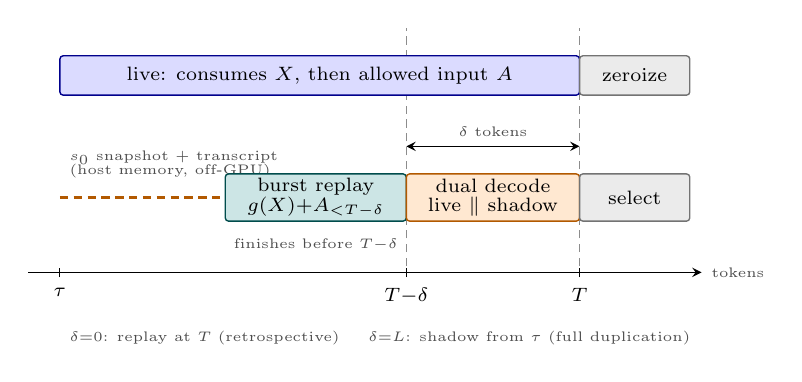
\begin{tikzpicture}[x=0.1mm,y=0.1mm,font=\scriptsize,>=stealth,
  live/.style={draw=blue!55!black,fill=blue!14,rounded corners=1.2pt,line width=0.5pt},
  shd/.style={draw=orange!70!black,fill=orange!18,rounded corners=1.2pt,line width=0.5pt},
  brs/.style={draw=teal!60!black,fill=teal!20,rounded corners=1.2pt,line width=0.5pt},
  gry/.style={draw=black!55,fill=black!8,rounded corners=1.2pt,line width=0.5pt},
  note/.style={font=\tiny,text=black!70}]
\def\xt{40}\def\xb{250}\def\xd{480}\def\xT{700}\def\xe{840}
% timeline
\draw[->,line width=0.5pt] (0,0) -- (\xe+15,0) node[right,note]{tokens};
\foreach \x/\l in {\xt/{$\tau$},\xd/{$T{-}\delta$},\xT/{$T$}}{\draw (\x,-6) -- (\x,6) node[below=4pt] {\l};}
\draw[densely dashed,black!45] (\xd,8) -- (\xd,310);
\draw[densely dashed,black!45] (\xT,8) -- (\xT,310);
% live branch
\draw[live] (\xt,225) rectangle (\xT,275);
\node at (370,250) {live: consumes $X$, then allowed input $A$};
\draw[gry] (\xT,225) rectangle (\xe,275);
\node at (770,250) {zeroize};
% shadow branch
\draw[densely dashed,orange!70!black,line width=0.8pt] (\xt,95) -- (\xb,95);
\node[note,anchor=south west,align=left] at (\xt,108) {$s_0$ snapshot $+$ transcript\\[-1pt](host memory, off-GPU)};
\draw[brs] (\xb,65) rectangle (\xd,125);
\node[align=center] at (365,95) {burst replay\\[-1pt]$g(X){+}A_{<T-\delta}$};
\draw[shd] (\xd,65) rectangle (\xT,125);
\node[align=center] at (590,95) {dual decode\\[-1pt]live $\Vert$ shadow};
\draw[gry] (\xT,65) rectangle (\xe,125);
\node at (770,95) {select};
\draw[<->,line width=0.5pt] (\xd,160) -- (\xT,160) node[midway,above,note]{$\delta$ tokens};
\node[note,anchor=north,align=center] at (365,55) {finishes before $T{-}\delta$};
\node[note,anchor=north west] at (\xt,-62) {$\delta{=}0$: replay at $T$ (retrospective) \hspace{2mm} $\delta{=}L$: shadow from $\tau$ (full duplication)};
\end{tikzpicture}
}
\caption{ShadowVeil with lookahead $\delta$. The $s_0$ snapshot and the transcript of allowed tokens wait in host
memory; fused bursts over the tokens observed so far build the shadow before $T{-}\delta$, the shadow then shares the batched decode step with
the live branch for $\delta$ tokens, and at $T$ the runtime selects it and zeroizes the live cache.}
\label{fig:overview}
\end{figure}

\begin{algorithm}[t]
\caption{ShadowVeil($\delta$): one revocation domain}
\label{alg:shadow}
\begin{algorithmic}[1]
\STATE \textbf{at} $\tau$: snapshot $s_0$ (host); start transcript of allowed tokens; live consumes $X$, then $A$
\STATE \textbf{at} release $r\le T{-}\delta$: allocate shadow cache $C\!\leftarrow\!s_0$; \textsc{Burst}: $C\!\leftarrow\!F^*_\theta(C,\,g(X)\|A_{<r})$ over the tokens observed so far, in idle-time chunks; replay tokens observed in $[r,T{-}\delta)$ the same way
\STATE \textbf{at} $T{-}\delta$: one catch-up chunk; \textbf{for} tokens in $[T{-}\delta,T)$ advance live and shadow in the \emph{same} batched decode step
\STATE \textbf{at} $T$: select $C$; zero every live-cache tensor; check $\max|\cdot|{=}0$; free $s_0$ and transcript
\STATE \textbf{if} $C$ not current at $T$: finish the remaining replay on the critical path (never more than the $\delta{=}0$ cost)
\end{algorithmic}
\end{algorithm}

\textbf{Cost.} Let $M$ be the fixed cache size, $L=|A|$ the authorized window (the tokens between $\tau$ and
$T$), so that the shadow performs $|g(X)|{+}L$ token transitions, and let $c_b$ be the per-token cost of
a fused burst. Replay-based exact reconstruction performs these $|g(X)|{+}L$ extra
transitions, the replay bound of \cite{executionunlearning}; state-transport shortcuts need a transport
criterion \cite{deltaomission}, and we claim no bound beyond replay. $\delta$ chooses \emph{when} and
\emph{where}. Only the $\Theta(M)$ retirement is independent of $L$ at the deadline; total work is always
$|g(X)|{+}L$. Retrospective replay pays $\approx(|g(X)|{+}L)\,c_b$ at $T$; a lookahead shadow pays
$(|g(X)|{+}L{-}\delta)c_b$ before $T{-}\delta$ plus $\delta$ decode rows, and holds a second $M$-byte cache
for $\delta$ plus the burst duration (peak $2M$, time-averaged residency about $(\delta/L)M$). The $s_0$
snapshot and the $O(L)$ transcript are a shared prerequisite of every exact method, held off the GPU until
release at the price of one host-to-device copy of $M$ bytes, a small fraction of a tick (not modeled).

\textbf{Deadline, lookahead and slack.} The policy states the expiry as a wall-clock deadline. The serving loop
advances in ticks of $\tau$~ms and each live session decodes one token per tick, so the token position $T$ of
the deadline is the number of ticks to it, and $\delta$ counts ticks before $T$. The \emph{burst slack} is the
idle part of the ticks between release and $T{-}\delta$: replay may stretch a tick to $1.5\tau$, leaving $1.5\tau$
minus the batched step. The shadow is current at $T{-}\delta$ when the replay queued
ahead of it in earliest-deadline order (the burst plus the backlog of tokens observed since release) fits in
that slack, and the release rule starts the burst as late as this allows (margin: three ticks). A token is
replayed only after it is observed. If the condition fails, the unfinished replay runs at $T$ and costs no more
than $\delta{=}0$.

\textbf{Burst from a non-zero snapshot.} The Hugging Face prefill branch zero-pads the convolution window, so
continuing a populated cache with several tokens ignores the previous $K{-}1$ inputs. We implement the burst
as a chunk that prepends the cached convolution window and initializes the scan from the cached SSM state.
Sec.~\ref{sec:mech} gives the deviations on real TAB prefixes ($s_0\neq0$).

\textbf{Exactness is path-relative.} Chunking moves where the fp32 scan state is rounded to fp16, and
batched kernels may pick different reduction orders. Different schedules therefore agree to $\sim$$10^{-3}$
but not bit for bit. Let a schedule $\Sigma$ fix the chunk boundaries, batch geometry, kernel configuration,
precision and cache layout. \emph{Proposition:} if the kernels are deterministic and a batched row's output does
not depend on its companion rows or its position, two executions of $\Sigma$ from the same $s_0$ and the same
tokens produce identical caches (induction over the operations of $\Sigma$). The guarantee is therefore bitwise
equality \emph{to a reference executed by the same recorded schedule and batch geometry}, which a deployment
enforces by logging $\Sigma$ with the transcript; across different schedules the agreement is numerical
(Sec.~\ref{sec:mech}), and the checks there test the row-independence assumption.

\section{Experimental Method}
\textbf{Data.} TAB contains 1{,}268 ECHR cases with entity annotations \cite{tab}; other annotated
identifiers are masked and eight real name surfaces are independently assigned to document-disjoint
contexts (counterfactual assignment, not natural pairings). Enron uses the CMU Enron-Meetings/Random subsets
with person-name annotations \cite{enronner}: 2{,}012 mentions in 720 documents, with one disjoint,
length-matched natural pseudonym as the class-independent sanitizer. Result files hold aggregates and hashes,
no names or passages.

\textbf{Models, probe, protocol.} Mamba-1 130M/370M/790M/1.4B and Mamba-2 130M/370M/780M, FP16, Transformers 4.51.3, PyTorch
2.5.1, CUDA 12.1. All timings, the protocol seeds of Table~\ref{tab:main} and the exactness checks ran on one RTX 3060 Laptop GPU (6 GB, power-capped, clocks not locked) with the host quiet (CPU load below 30\%); the 1.4B and Mamba-2 attacker audits, the nonlinear probes and the counterfactual-distance runs ran on an RTX 3050 (8 GB), with no timings taken there and each result from a single machine. Eight seeds, 20261001--8 (96 attacker-training and 48 test documents per seed, balanced
over eight identities, no overlap within a seed; each seed draws its contexts and name assignment independently from the corpus pool, so seeds are resamples that may share documents); the first three were prespecified for the decision rule. The primary
probe is a standardized ridge classifier ($\alpha{=}10$) on 24{,}576 seeded SSM coordinates measured after a
fixed neutral continuation, retrained per condition; a second label embedded in allowed text measures
retained-state utility. Prespecified decision rule: all equality checks pass, mean shadow
identity accuracy $\le$18.75\% (chance plus half a class), retained accuracy not significantly lower.

\textbf{Controls and instrumentation.} (a) A \emph{leaky sanitizer} that keeps the first three characters of the
name; (b) a ridge probe on the \emph{full} cache (all SSM and convolution state) and a training-free
\emph{logit-access} attacker that scores each candidate name by its log-likelihood under the cache (a white-box audit
oracle that holds the weights, stronger than the state-only adversary); (c) a
label-permutation null for the ridge probe and seed-level TOST equivalence tests with a margin of 6.25 points (half a class); (d) Mamba-2 with the same attacker protocol.

\section{Results}
\subsection{Mechanism: exact counterfactual state equality}\label{sec:mech}
Every equality and zeroization check passes. Boundary and continuation equality hold for both corpora at three scales
(Sec.~\ref{sec:audit}), and an online runtime on eight real TAB streams (live 98--142, sanitized 99--137 tokens) selects caches equal to
separately allocated sanitized sessions at expiry and after continuation. On the fused path the shadow equals its independently
rebuilt reference at every offset $\delta$, endpoints included, and on seven further documents per scale ($\nExtraExactA$/$\nExtraNA$
offset--document checks at each of 130M, 370M and 1.4B); the runtime's counter of executed transitions equals $|g(X)|{+}L$ for every
shadow, so conservation is counted, not derived. From non-zero snapshots ($s_0\neq0$ after a real TAB prefix) the chunked burst is
bitwise equal to its reference in $\nKOneExactA/\nKOneNA$ (130M), $\nKOneExactB/\nKOneNB$ (370M) and $\nKOneExactC/\nKOneNC$ (1.4B)
cases. It differs from a monolithic prefill of the sanitized stream by at most $\nKOneMonoB\%$ of the state magnitude and from the
token-by-token recurrence by at most $\nKOneChunkRecB\%$, while live and sanitized states differ by at least $\nKOneSignalB\%$; a
burst through the prefill branch deviates by $\nKOneNaiveLoB$--$\nKOneNaiveHiA\%$, comparable to the signal being removed. Batched
rows are deterministic and independent of the companion row and of row position,
so a reference built in the same geometry reproduces the shadow row bitwise at every offset and scale.
\begin{table}[t]
\caption{Identity recovery (lower is better) and retained-label accuracy, untreated $\to$ ShadowVeil (\%; mean $\pm$ SD over eight
seeds; chance 12.5\%). TOST: equivalence to chance within $\pm6.25$ points, seed level; full reset gives 12.5/12.5.}
\label{tab:main}
\centering
\resizebox{\columnwidth}{!}{%
\begin{tabular}{llrrr}
\toprule
Model & Corpus & Identity & Retained & TOST $p$ \\
\midrule
130M & TAB & $\nTUTabA\pm\nTUTabASd\to\nTSTabA\pm\nTSTabASd$ & $\nTRUTabA\to\nTRSTabA$ & $\nEqTabAP$ \\
130M & Enron & $\nTUEnronA\pm\nTUEnronASd\to\nTSEnronA\pm\nTSEnronASd$ & $\nTRUEnronA\to\nTRSEnronA$ & $\nEqEnronAP$ \\
370M & TAB & $\nTUTabB\pm\nTUTabBSd\to\nTSTabB\pm\nTSTabBSd$ & $\nTRUTabB\to\nTRSTabB$ & $\nEqTabBP$ \\
370M & Enron & $\nTUEnronB\pm\nTUEnronBSd\to\nTSEnronB\pm\nTSEnronBSd$ & $\nTRUEnronB\to\nTRSEnronB$ & $\nEqEnronBP$ \\
790M & TAB & $\nTUTabD\pm\nTUTabDSd\to\nTSTabD\pm\nTSTabDSd$ & $\nTRUTabD\to\nTRSTabD$ & $\nEqTabDP$ \\
790M & Enron & $\nTUEnronD\pm\nTUEnronDSd\to\nTSEnronD\pm\nTSEnronDSd$ & $\nTRUEnronD\to\nTRSEnronD$ & $\nEqEnronDP$ \\
1.4B & TAB & $\nTUTabC\pm\nTUTabCSd\to\nTSTabC\pm\nTSTabCSd$ & $\nTRUTabC\to\nTRSTabC$ & $\nEqTabCP$ \\
1.4B & Enron & $\nTUEnronC\pm\nTUEnronCSd\to\nTSEnronC\pm\nTSEnronCSd$ & $\nTRUEnronC\to\nTRSEnronC$ & $\nEqEnronCP$ \\
\bottomrule
\end{tabular}}
\end{table}

\subsection{Measured costs on a fused path}\label{sec:fused}
The fused path runs a decode step as one CUDA graph and a burst as one Triton scan over the chunk (Sec.~III); it agrees with the
Hugging Face path to $\nFusedHFDiffA/\nFusedHFDiffB/\nFusedHFDiffC\%$ of the state magnitude (130M/370M/1.4B). On an RTX 3060 Laptop
GPU, measured on a quiet host, a decode step takes $\nStepOneA/\nStepOneB/\nStepOneC$ ms and one more batched row adds
$\nBatchMarginLoB$--$\nBatchMarginHiA\%$ of a live step at batch 2. A burst of 256 tokens takes $\nChunkSmallA/\nChunkSmallB/\nChunkSmallC$ ms and
grows linearly with the window ($\nChunkLargeA$ ms for 8{,}192 tokens at 130M), about $\nStepPerChunkTokA\times$ cheaper per token than
decoding. Against the official \texttt{mamba\_ssm} kernel on the same GPU, our scan takes $\nScanOneOursA$ against $\nScanOneOfficialA$ ms per layer for one token at 130M and $\nScanTwoFiftySixOursA$ against $\nScanTwoFiftySixOfficialA$ ms over 256 tokens (the official parallel scan starts from a zero state), so the burst costs are conservative. Retirement is one grouped zeroing call of $\nRetireGroupedA$--$\nRetireGroupedB$ ms ($\nRetireA$--$\nRetireC$ ms as a per-tensor
loop); the host-side max-abs check is an audit step that runs after the shadow is selected.
Replay at the deadline for a 256-token window therefore costs $\nBurstZeroA/\nBurstZeroB/\nBurstZeroC$ ms against $\nRetireGroupedA$ ms for
selecting the shadow and zeroing the live cache, and it grows with window length and model size while retirement does not. Work
is conserved in transitions but not in time: decoding a shadow alone for the whole window costs $\nTotalFullA$ ms of extra compute
at 130M ($\delta{=}L$) against $\nBurstZeroA$ ms for one burst ($\delta{=}0$), so the useful setting is a short lookahead (Sec.~\ref{sec:sim}).

\subsection{Scheduler simulation and serving harness}\label{sec:sim}
We drive a tick-based scheduler ($\tau=\nSimTauA$~ms at 130M and 370M) with the measured per-scale costs: the decode step at every measured batch size
(up to 512, 192 and 96 rows at 130M, 370M and 1.4B, within a 1.5~GB budget for stacked live and shadow cache; beyond that the last measured slope is extended),
interpolated chunk cost, and grouped retirement. Sessions arrive as a Poisson process whose rate sets the concurrency, with windows
uniform in 128--256 tokens, a fraction of the expiries aligned to a common boundary, and one token per session per tick. Replay chunks hold at most 32 tokens in the simulation and 64 in the harness
(64 for the final catch-up), do not preempt, and run in the idle part of a tick; expiries in one tick serialize. An earliest-deadline release rule spends only the idle part of each tick on shadow bursts.
Cache memory counts the per-session recurrent caches; weights, allocator slack and burst workspace (largest for replay at the deadline, which bursts the whole window) are excluded.
Retrospective replay (\emph{retro}) does all work at the deadline; \emph{star} uses $\delta^\star=\lceil\text{burst}/\tau\rceil+1$;
\emph{la16} and \emph{la50} hold a fixed lookahead of 16 tokens and of half the window; \emph{full} duplicates throughout.

\begin{figure*}[t]
\centering
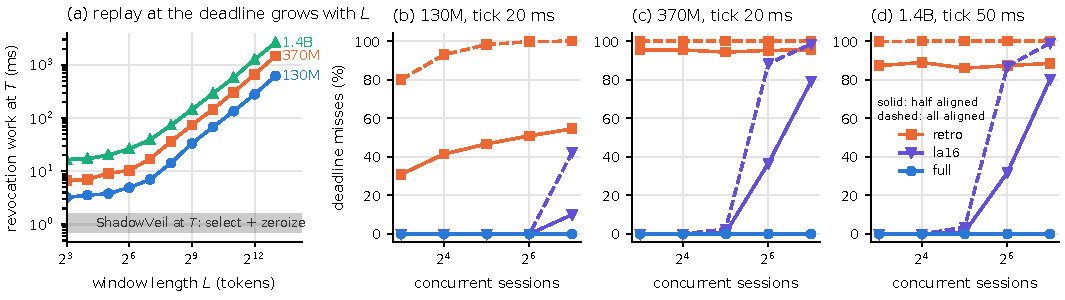
\includegraphics[width=0.92\textwidth]{fig_cost_sched}
\caption{(a) Work left at the deadline by replay grows with the window $L$ and with model size, while ShadowVeil's selection and zeroizing at $T$ costs about a millisecond. (b--d) Simulated deadline-miss rate (SLO: one tick) against concurrent sessions, from measured costs: retrospective replay (retro), a 16-token lookahead (la16) and full duplication (full), with half of the expiries aligned (solid) or all aligned (dashed).}
\label{fig:sched}
\end{figure*}


\begin{table}[t]
\caption{Revocation latency p99 (ms) / deadline-miss rate (SLO: one tick) and mean cache (MB) under measured costs, tick $\tau=20$~ms (130M, 370M) and 50~ms (1.4B, whose batched step exceeds 20~ms). Typical load: 16 sessions, half of the expiries aligned. Extreme load: 64 sessions all expiring together.}
\label{tab:sched}
\centering
\resizebox{\columnwidth}{!}{%
\begin{tabular}{lrrrrr}
\toprule
 & retro & star & la16 & la50 & full \\
\midrule
\multicolumn{6}{l}{\emph{typical load}} \\
130M & \nTypRetroPNinetyNineA\,/\,\nTypRetroMissA\% & \nTypStarPNinetyNineA\,/\,\nTypStarMissA\% & \nTypLaSixteenPNinetyNineA\,/\,\nTypLaSixteenMissA\% & \nTypLaHalfPNinetyNineA\,/\,\nTypLaHalfMissA\% & \nTypFullPNinetyNineA\,/\,\nTypFullMissA\% \\
\quad cache MB & \nTypRetroMemA & \nTypStarMemA & \nTypLaSixteenMemA & \nTypLaHalfMemA & \nTypFullMemA \\
370M & \nTypRetroPNinetyNineB\,/\,\nTypRetroMissB\% & \nTypStarPNinetyNineB\,/\,\nTypStarMissB\% & \nTypLaSixteenPNinetyNineB\,/\,\nTypLaSixteenMissB\% & \nTypLaHalfPNinetyNineB\,/\,\nTypLaHalfMissB\% & \nTypFullPNinetyNineB\,/\,\nTypFullMissB\% \\
\quad cache MB & \nTypRetroMemB & \nTypStarMemB & \nTypLaSixteenMemB & \nTypLaHalfMemB & \nTypFullMemB \\
1.4B & \nTypRetroPNinetyNineC\,/\,\nTypRetroMissC\% & \nTypStarPNinetyNineC\,/\,\nTypStarMissC\% & \nTypLaSixteenPNinetyNineC\,/\,\nTypLaSixteenMissC\% & \nTypLaHalfPNinetyNineC\,/\,\nTypLaHalfMissC\% & \nTypFullPNinetyNineC\,/\,\nTypFullMissC\% \\
\quad cache MB & \nTypRetroMemC & \nTypStarMemC & \nTypLaSixteenMemC & \nTypLaHalfMemC & \nTypFullMemC \\
\midrule
\multicolumn{6}{l}{\emph{extreme load}} \\
130M & \nSimRetroPNinetyNineA\,/\,\nSimRetroMissA\% & \nSimStarPNinetyNineA\,/\,\nSimStarMissA\% & \nSimLaSixteenPNinetyNineA\,/\,\nSimLaSixteenMissA\% & \nSimLaHalfPNinetyNineA\,/\,\nSimLaHalfMissA\% & \nSimFullPNinetyNineA\,/\,\nSimFullMissA\% \\
\quad cache MB & \nSimRetroMemA & \nSimStarMemA & \nSimLaSixteenMemA & \nSimLaHalfMemA & \nSimFullMemA \\
370M & \nSimRetroPNinetyNineB\,/\,\nSimRetroMissB\% & \nSimStarPNinetyNineB\,/\,\nSimStarMissB\% & \nSimLaSixteenPNinetyNineB\,/\,\nSimLaSixteenMissB\% & \nSimLaHalfPNinetyNineB\,/\,\nSimLaHalfMissB\% & \nSimFullPNinetyNineB\,/\,\nSimFullMissB\% \\
\quad cache MB & \nSimRetroMemB & \nSimStarMemB & \nSimLaSixteenMemB & \nSimLaHalfMemB & \nSimFullMemB \\
1.4B & \nSimRetroPNinetyNineC\,/\,\nSimRetroMissC\% & \nSimStarPNinetyNineC\,/\,\nSimStarMissC\% & \nSimLaSixteenPNinetyNineC\,/\,\nSimLaSixteenMissC\% & \nSimLaHalfPNinetyNineC\,/\,\nSimLaHalfMissC\% & \nSimFullPNinetyNineC\,/\,\nSimFullMissC\% \\
\quad cache MB & \nSimRetroMemC & \nSimStarMemC & \nSimLaSixteenMemC & \nSimLaHalfMemC & \nSimFullMemC \\
\bottomrule
\end{tabular}}
\end{table}

Figure~\ref{fig:sched} shows the miss rate against load. At a typical load a 16-token lookahead removes the deadline misses at every scale (p99 \nTypLaSixteenPNinetyNineA, \nTypLaSixteenPNinetyNineB{} and \nTypLaSixteenPNinetyNineC~ms at 130M, 370M and 1.4B) for \nTypLaSixteenMemA, \nTypLaSixteenMemB{} and \nTypLaSixteenMemC~MB of mean cache against \nTypRetroMemA, \nTypRetroMemB{} and \nTypRetroMemC~MB for replay at the deadline, which misses \nTypRetroMissA\%, \nTypRetroMissB\% and \nTypRetroMissC\% of deadlines; full duplication uses \nTypFullMemA, \nTypFullMemB{} and \nTypFullMemC~MB. Under extreme load the benefit depends on scale. At 130M a
16-token lookahead still removes every miss (p99 \nSimLaSixteenPNinetyNineA~ms). At 370M and 1.4B the batched decode step for 64 sessions occupies most of a tick, so the schedule matches the lookahead to the idle time: a half-window lookahead cuts the misses from \nSimRetroMissB\% and \nSimRetroMissC\% to \nSimLaHalfMissB\% and \nSimLaHalfMissC\%, and full duplication meets every deadline, at about twice the memory of replay.
The burst-time rule \emph{star}, the smallest lookahead that hides one burst, suffices at 130M typical load; elsewhere the longer fixed lookaheads are needed (Table~\ref{tab:sched}), so the lookahead is set from the measured costs at each scale and load.

\emph{Serving harness.} The same workloads and policies run on the GPU, with the decode batch sized to the load and every burst, decode step and retirement executed for real. At 130M, 370M and 1.4B the harness and the simulation agree on whether a policy meets its deadline in $\nSvhSloA\%$, $\nSvhSloB\%$ and $\nSvhSloC\%$ of \nSvhConfigsA, \nSvhConfigsB{} and \nSvhConfigsC{} configurations, predict the mean cache memory with a median error of about 2\%, and rank the policies by p99 latency with Spearman correlation $\nSvhSpearmanA$, $\nSvhSpearmanB$ and $\nSvhSpearmanC$. The simulation understates the latency of replay at the deadline, by a median factor of \nSvhMedRatioA, \nSvhMedRatioB{} and \nSvhMedRatioC, so the measured benefit of lookahead is larger than the simulated one. In the harness a 16-token lookahead removes every miss at 16 sessions with half the expiries aligned at 130M, 370M and 1.4B, where replay at the deadline misses most or all deadlines.
\emph{Cost to co-resident sessions.} In the same harness runs (typical load, no arrivals dropped) replay at the deadline stalls the whole batch, so a 16-token lookahead
shortens the p99 tick from \nHarTickRetroA, \nHarTickRetroB{} and \nHarTickRetroC~ms to \nHarTickLaSixteenA, \nHarTickLaSixteenB{} and \nHarTickLaSixteenC~ms at 130M, 370M and 1.4B, and the mean tick relative to nominal from
\nHarSlowRetroA, \nHarSlowRetroB{} and \nHarSlowRetroC{} to \nHarSlowLaSixteenA, \nHarSlowLaSixteenB{} and \nHarSlowLaSixteenC; full duplication gives \nHarTickFullA, \nHarTickFullB{} and \nHarTickFullC~ms.
Miss rates compare policies within a scale, since the tick differs across scales.

\subsection{Comparison with baselines}
Table~\ref{tab:compare} summarizes the alternatives: only replay and ShadowVeil reach the sanitized state, and ShadowVeil is the one whose deadline work is a selection and a zeroing call.
Yao et al.\ give a lower bound of $T-\tau+1$ recomputed transitions for exact revocation by sanitized replay, for a session of length $T$ whose target entered at
step $\tau$. ShadowVeil performs exactly the replay transitions at every $\delta$ (counted in our sweep) and changes only \emph{when} they run.
We implement replay at the deadline following their method as the baseline; approximate unlearning and state-editing baselines do not give state equality (Sec.~\ref{sec:audit}). The release rule (earliest deadline first over the idle budget, with $\delta^\star$ set from the burst time) is itself a deadline-aware replay scheduler, and la16, la50 and full fix how much of the window the shadow rides along the batched step, so the comparison contains proactive replay at several operating points. Against a
Transformer, whose cache grows with context (GPT-2: 18.9~MB at 512 tokens), one Mamba-130M cache is
1.47~MB at any length, so a full shadow costs a constant for fixed-state models. \emph{Distance to the counterfactual.} Following Yao et al., we measure how far each treated state is from the state of the sanitized-stream execution, by relative state distance, next-token KL, and the fraction of matched-seed generations identical to the counterfactual's. At 130M (\nCfdSeedsA{} seeds) the untreated state is at distance $\nCfdUntreatedDistA$ with KL $\nCfdUntreatedKlA$ and reproduces the counterfactual generation in $\nCfdUntreatedGenIdA\%$ of draws. A full reset moves it to $\nCfdResetDistA$ (KL $\nCfdResetKlA$, $\nCfdResetGenIdA\%$ identical), and a sensitive-subspace edit leaves it at $\nCfdSubspaceDistA$ (KL $\nCfdSubspaceKlA$, $\nCfdSubspaceGenIdA\%$), no closer than doing nothing and no closer than a random subspace of the same rank ($\nCfdRandomDistA$, $\nCfdRandomGenIdA\%$). The ShadowVeil state is at distance $\nCfdShadowDistA$ (KL below $10^{-6}$) and every generation is identical. Replay at the deadline reaches the same state; the two differ in when the work runs (Sec.~\ref{sec:sim}).

\begin{table}[t]
\caption{Revocation methods side by side (130M, TAB). Identity recovery is the strongest attacker's accuracy (chance 12.5\%); work at the deadline is the cost of producing the revoked state at $T$ for a 256-token window.}
\label{tab:compare}
\centering
\resizebox{\columnwidth}{!}{%
\begin{tabular}{lccc}
\toprule
Method & Equals sanitized state & Identity recovery (\%) & Work at deadline (ms) \\
\midrule
Untreated & no & \nAudUntreatedLogitA & 0 \\
Full reset & no (context lost) & 12.5 & $<$1 \\
Subspace edit & no & 62.5 & $<$1 \\
Replay at the deadline & yes & \nAudPrimaryLogitA & \nBurstZeroA \\
ShadowVeil & yes & \nAudPrimaryLogitA & \nRetireGroupedA \\
\bottomrule
\end{tabular}}
\end{table}

\subsection{Sanitizer audit and attackers}\label{sec:audit}
In these corpora the sanitized stream carries no class signal by construction (one class-independent placeholder or pseudonym) and names are
assigned to contexts independently of content, so near-chance recovery follows from state equality. The attacker results are therefore controls on the
equality guarantee: untreated states are the positive control, a full reset the negative control and the leaky sanitizer the sanitizer audit. They are
not independent evidence of identity privacy beyond the sanitizer; an identity that retained context reveals (occupation, location) is sanitizer-and-context
leakage, which a corpus with natural name--context correlations would measure. Across eight seeds per cell
(Table~\ref{tab:main}) the shadow state is equivalent to chance within half a class (TOST, seed level) in seven of eight (scale, corpus)
cells ($p\le0.012$); the eighth, 130M TAB, has mean $\nEqTabAMean\%$ (95\% CI $[\nEqTabALo,\nEqTabAHi]$), inside the prespecified bound of
$18.75\%$ ($p=\nEqTabAP$). The equivalence margin is half a class, a statement about these classifiers and not a formal privacy bound, and the seed-level test treats the
eight resamples as exchangeable. Retained-label accuracy is preserved: the paired seed-level difference (ShadowVeil minus untreated) lies between $\nRetDiffLo$ and $+\nRetDiffHi$ points over the
\nRetCells{} cells, and its one-sided 95\% lower bound exceeds $-6.25$ points in \nRetNIOk{} of them (the exception, 1.4B Enron, has a bound of $\nRetNIWorstBound$ at 48 test documents per seed), whereas a full reset
reaches chance on both labels.

\begin{table}[t]
\caption{Four attackers on untreated, ShadowVeil (class-independent sanitizer) and a leaky sanitizer that keeps three characters of
the name; identity accuracy (\%, 130M, mean of eight seeds, chance 12.5). Bitwise equality to the declared sanitized stream holds in
every run, for both sanitizers.}
\label{tab:attackers}
\centering
\resizebox{\columnwidth}{!}{%
\begin{tabular}{lrrrrrr}
\toprule
 & \multicolumn{3}{c}{TAB} & \multicolumn{3}{c}{Enron} \\
\cmidrule(lr){2-4}\cmidrule(lr){5-7}
Attacker & Untr. & ShadowVeil & Leaky & Untr. & ShadowVeil & Leaky \\
\midrule
Ridge, seeded coordinates & \nAudUntreatedRidgeA & \nAudPrimaryRidgeA & \nAudLeakyRidgeA & \nEAudUntreatedRidgeA & \nEAudPrimaryRidgeA & \nEAudLeakyRidgeA \\
Ridge, full cache & \nAudUntreatedFullA & \nAudPrimaryFullA & \nAudLeakyFullA & \nEAudUntreatedFullA & \nEAudPrimaryFullA & \nEAudLeakyFullA \\
Logit access (candidate scoring) & \nAudUntreatedLogitA & \nAudPrimaryLogitA & \nAudLeakyLogitA & \nEAudUntreatedLogitA & \nEAudPrimaryLogitA & \nEAudLeakyLogitA \\
Logit access, best of six probes & \nAudUntreatedLogitBestA & \nAudPrimaryLogitBestA & \nAudLeakyLogitBestA & \nEAudUntreatedLogitBestA & \nEAudPrimaryLogitBestA & \nEAudLeakyLogitBestA \\
\bottomrule
\end{tabular}}
\end{table}

The logit-access attacker recovers the name from $\nAudUntreatedLogitA\%$ (TAB) and $\nEAudUntreatedLogitA\%$ (Enron) of untreated
states, a strong positive control. On the ShadowVeil state all four attackers stay at chance (the best-of-six value is a maximum of
six noisy readings and is expected to sit above 12.5). The leaky-sanitizer control confirms that the guarantee is equality to the declared
sanitizer: equality is exact in all $\nAuditExactA$ seeds, and recovery rises to $\nAudLeakyLogitA\%$ (TAB) and $\nEAudLeakyLogitA\%$ (Enron)
because that sanitizer keeps part of the name. At 370M the same pattern holds
(logit access on the leaky sanitizer: $\nAudLeakyLogitB\%$ TAB, $\nEAudLeakyLogitB\%$ Enron). At 1.4B the logit-access attacker recovers
the name from $\nAudUntreatedLogitC\%$ (TAB) and $\nEAudUntreatedLogitC\%$ (Enron) of untreated states, $\nAudPrimaryLogitC\%$ and
$\nEAudPrimaryLogitC\%$ on the ShadowVeil state, and $\nAudLeakyLogitC\%$ and $\nEAudLeakyLogitC\%$ on the leaky sanitizer.

\emph{Mamba-2.} The same protocol runs on Mamba-2 (SSD) at 130M, 370M and 780M, with a window of \nMtwoWindowA{} tokens: the shadow cache
equals the independently executed sanitized reference bitwise at all \nMtwoDeltasA{} lookahead offsets and at the deadline boundary at every
size, and the retired cache is exactly zero. With the seeded-coordinate attacker, identity recovery falls from $\nMtwoUntreatedA\%$,
$\nMtwoUntreatedB\%$ and $\nMtwoUntreatedD\%$ on untreated states to $\nMtwoShadowA\%$, $\nMtwoShadowB\%$ and $\nMtwoShadowD\%$ on
the ShadowVeil state (chance 12.5\%; \nMtwoSeedsA, \nMtwoSeedsB{} and \nMtwoSeedsD{} seeds at 130M, 370M and 780M), while retained-label
accuracy stays at $\nMtwoRetSA\%$, $\nMtwoRetSB\%$ and $\nMtwoRetSD\%$ (untreated: $\nMtwoRetUA\%$, $\nMtwoRetUB\%$, $\nMtwoRetUD\%$).

Nonlinear probes do not change the picture. On the full cache, a two-layer MLP and a sparse-autoencoder probe recover the name from $\nStrongUntreatedMlpA\%$ and $\nStrongUntreatedSaeA\%$ of untreated states at 130M (linear probe: $\nStrongUntreatedLinearA\%$) and from $\nStrongShadowMlpA\%$ and $\nStrongShadowSaeA\%$ on the ShadowVeil state (\nStrongSeedsA{} seeds; 370M: $\nStrongShadowMlpB\%$ and $\nStrongShadowSaeB\%$; 1.4B: $\nStrongShadowMlpC\%$ and $\nStrongShadowSaeC\%$), at chance.

Subspace editing, the usual approximate alternative, leaves the identity recoverable. Identity recovery on the edited coordinates falls from 89.6\% to 60.4\%,
but a disjoint coordinate view of the same layers retains 81.3\% and the combined attacker obtains 62.5\%; editing the selected
layers fully still permits 52.1\% combined recovery. With identities disjoint between defense training and evaluation, a rank-32
subspace changes recovery only from 97.9\% to 93.8\%, and rank 127 leaves it at 97.9\%.

\subsection{Multi-item revocation}\label{sec:multi}
An eager exact construction for a session with $k$ items whose revocation order is unknown keeps one branch per subset of items that may be revoked
inside the same ambiguity window $w$, so its live branch count is $2^w$, not $2^k$. We exercised $k\le6$ items with windows up to
$w=6$ ($\nMultiNA$ configurations per scale): each branch, on reveal, equals its reference bitwise at 130M, 370M and 1.4B
($\nMultiExactA/\nMultiNA$ at each scale). The largest case held $\nMultiMaxBranchesA$ branches, \nMultiMaxMBA~MB at 130M,
\nMultiMaxMBB~MB at 370M and \nMultiMaxMBC~MB at 1.4B; branch memory grows exponentially in $w$ and linearly in state size, which is the
practical limit. This is the construction with every subset's state ready; lazy or compressed representations trade readiness for replay time ($\delta{=}0$), and we claim no bound for them. When the deadline order is known, irreversible deadline masks form a nested chain of at most $b+1$ states for $b$
distinct deadline buckets (exhaustively checked over 3,279 assignments, no violations), so a known order needs $b+1$ rather than
$2^w$ branches.

\section{Discussion and Scope}\label{sec:limits}
The guarantee is equality to a declared sanitized execution, so privacy is that of the sanitizer, as the leaky-sanitizer control shows (Sec.~\ref{sec:audit}),
and of the transcript it is applied to: the target is the sanitized state continued by the recorded authorized transcript $A$ (transcript-conditioned revocation),
not a regenerated trajectory. Content in $A$ that derives from $X$, such as a reply that repeats a revoked value, stays in the sanitized state as the retained part of a name does in the leaky control,
so such spans are declared part of the revoked set (Sec.~\ref{sec:multi}); regenerating replies under $g(X)$ is a separate problem.
Zeroization is verified on the declared cache tensors (SSM and convolution state, max-abs zero); transient workspace, allocator memory, CUDA-graph pools, host copies and logged transcripts need system-level scrubbing outside this evaluation.
Exactness holds for a fixed schedule and batch geometry, and batched rows are deterministic and independent of their companions. A shadow row raises a batched step by $\nBatchMarginLoB$--$\nBatchMarginHiA\%$, and a full-window shadow costs about
40$\times$ the compute of one burst at 130M, so a short lookahead is the efficient setting.
All measurements come from two consumer-grade GPUs, a power-capped 6~GB laptop part and an 8~GB desktop part, so the study covers models of up to 1.4B
parameters (Mamba-2 up to 780M) and batches of about a hundred sessions on a single device. Absolute times belong to that hardware and the comparison between schedules
is the portable result; on production kernels, datacenter-class GPUs and larger models the lookahead is re-measured and set from the same cost model.
The workloads are synthetic expiry patterns with one token per session per tick; stochastic expiry distributions, prefill--decode mixing, preemption and variable decode rates are the next workloads for the same cost model.
ShadowVeil targets one revocation domain per session; with $w$ order-ambiguous items the eager construction holds $2^w$ branches, and a known order needs only $b+1$.

\section{Conclusion}
ShadowVeil keeps the exact transition count of replay and moves it ahead of the deadline, with bitwise equality to a sanitized
reference run under the same recorded schedule at every lookahead, from non-zero snapshots and on Mamba-1 and Mamba-2. A 16-token lookahead
removes the deadline misses at 16 sessions with half the expiries aligned at 130M, 370M and 1.4B; under extreme load at 370M and 1.4B full duplication meets every deadline. Identity
recovery falls from \nTUTabA\% to \nTSTabA\% (TAB, eight seeds), with a leaky-sanitizer control
delimiting the guarantee. Future work is a production-kernel path, datacenter-class hardware and larger models. Code, measurements and the verification script are available at \texttt{github.com/\allowbreak{}AbdelrahmanAboegela/\allowbreak{}ShadowVeil}.

\section*{Acknowledgment}
The authors used Anthropic Claude to assist with figure and table preparation, \LaTeX{} formatting, language proofreading, and improving the structure and organization of existing code. All AI-assisted outputs were reviewed and verified by the authors, who take full responsibility for the manuscript's content.

\begin{thebibliography}{12}
\scriptsize
\setlength{\itemsep}{0pt}
\setlength{\parskip}{0pt}
\setlength{\parsep}{0pt}
\bibitem{mamba}
A. Gu and T. Dao, ``Mamba: Linear-time sequence modeling with selective state spaces,'' arXiv:2312.00752, 2023.

\bibitem{mamba2}
T. Dao and A. Gu, ``Transformers are SSMs: Generalized models and efficient algorithms through structured state space duality,'' in \emph{Proc. ICML}, 2024.

\bibitem{mambamemory}
T. Hossain et al., ``Characterizing Mamba's selective memory using auto-encoders,'' in \emph{Proc. IJCNLP-AACL}, 2025.

\bibitem{coavoux}
M. Coavoux, S. Narayan, and S. B. Cohen, ``Privacy-preserving neural representations of text,'' in \emph{Proc. EMNLP}, 2018.

\bibitem{embeddings}
J. Morris, V. Kuleshov, V. Shmatikov, and A. Rush, ``Text embeddings reveal (almost) as much as text,'' in \emph{Proc. EMNLP}, 2023.

\bibitem{executionunlearning}
C. Yao et al., ``Forgetting without restarting: Execution-state unlearning for stateful LLM agents,'' arXiv:2609.04875, 2026.

\bibitem{attriguard}
Y. He et al., ``AttriGuard: Defeating indirect prompt injection in LLM agents via causal attribution of tool invocations,'' in \emph{Proc. USENIX Security Symp.}, 2026.

\bibitem{cacheprune}
G. Wu et al., ``CachePrune: Privacy-aware and fine-grained KV cache sharing for efficient LLM inference,'' arXiv:2605.23640, 2026.

\bibitem{shadowcache}
Z. Luo et al., ``Shadow in the cache: Unveiling and mitigating privacy risks of KV-cache in LLM inference,'' in \emph{Proc. NDSS}, 2026.

\bibitem{ready2unlearn}
H. Duan, Y. Yang, A. Abbasi, and K. Y. Tam, ``Ready2Unlearn: A learning-time approach for preparing models with future unlearning readiness,'' arXiv:2505.10845, 2025.

\bibitem{replayssm}
Z.-W. Liou et al., ``ReplaySSM: Cache SSM inputs, not state,'' arXiv:2610.13778, 2026.

\bibitem{marconi}
R. Pan et al., ``Marconi: Prefix caching for the era of hybrid LLMs,'' in \emph{Proc. MLSys}, 2025.

\bibitem{tab}
I. Pil\'{a}n et al., ``The Text Anonymization Benchmark (TAB): A dedicated corpus and evaluation framework for text anonymization,'' \emph{Computational Linguistics}, vol. 48, no. 4, 2022.

\bibitem{enronner}
E. Minkov, R. C. Wang, and W. W. Cohen, ``Extracting personal names from email: Applying named entity recognition to informal text,'' in \emph{Proc. HLT/EMNLP}, 2005.

\bibitem{deltaomission}
V. Ramesh, ``Exact record omission in delta attention: A transport criterion, its cost, and a replay certificate,'' arXiv:2609.06872, 2026.

\bibitem{congestion}
R. Ao et al., ``Service-induced congestion in memory-constrained LLM serving,'' arXiv:2606.15555, 2026.

\bibitem{eraser}
Y. Hu et al., ``ERASER: Machine unlearning in MLaaS via an inference serving-aware approach,'' in \emph{Proc. ACM CCS}, 2024.

\end{thebibliography}

\end{document}
